%%%%%%%%%%%%%%%%%%%%%%%%%%%%%%%%%%%%%%%%
% datoteka diploma-FRI-vzorec.tex
%
%POZOR: ta verzija ne producira pdf datoteke v pdf/A formatu!!!
%namenjena je le za nalogo pri Diplomskem seminarju!
%
% vzorčna datoteka za pisanje diplomskega dela v formatu LaTeX
% na UL Fakulteti za računalništvo in informatiko
%
% na osnovi starejših verzij vkup spravil Franc Solina, maj 2021
% prvo verzijo je leta 2010 pripravil Gašper Fijavž
%
% za upravljanje z literaturo ta vezija uporablja BibLaTeX
%
% svetujemo uporabo Overleaf.com - na tej spletni implementaciji LaTeXa ta vzorec zagotovo pravilno deluje
%
\documentclass[a4paper,12pt,openright]{book}
%\documentclass[a4paper, 12pt, openright, draft]{book}  Nalogo preverite tudi z opcijo draft, ki pokaže, katere vrstice so predolge! Pozor, v draft opciji, se slike ne pokažejo!
 
\usepackage[utf8]{inputenc}   % omogoča uporabo slovenskih črk kodiranih v formatu UTF-8
\usepackage[slovene,english]{babel}    % naloži, med drugim, slovenske delilne vzorce
\usepackage[pdftex]{graphicx}  % omogoča vlaganje slik različnih formatov
\usepackage{fancyhdr}          % poskrbi, na primer, za glave strani
\usepackage{amssymb}           % dodatni matematični simboli
\usepackage{amsmath}           % eqref, npr.
\usepackage[pdftex, colorlinks=true,
						citecolor=black, filecolor=black, 
						linkcolor=black, urlcolor=black,
						pdfproducer={LaTeX}, pdfcreator={LaTeX}]{hyperref}
\usepackage{hyperxmp}
\usepackage{csquotes}

\usepackage{color}
\usepackage{soul}

\usepackage{comment}
\usepackage{float}

\usepackage{algorithm}
\usepackage{algpseudocode}


\usepackage{amsmath} % for aligned
\usepackage{listofitems} % for \readlist to create arrays
\usepackage{tikz}
\usetikzlibrary{arrows.meta} % for arrow size
\usetikzlibrary{fit}
\usepackage[outline]{contour} % glow around text
\contourlength{1.4pt}

% COLORS
\usepackage{xcolor}
\colorlet{myred}{red!80!black}
\colorlet{myblue}{blue!80!black}
\colorlet{mygreen}{green!60!black}
\colorlet{myorange}{orange!70!red!60!black}
\colorlet{mydarkred}{red!30!black}
\colorlet{mydarkblue}{blue!40!black}
\colorlet{mydarkgreen}{green!30!black}
\colorlet{mydarkorange}{orange!30!black}
\colorlet{softorange}{orange!80}

\definecolor{errorred}{RGB}{204, 0, 0}
\definecolor{softerrorred}{RGB}{220, 20, 60}

% STYLES
\tikzset{
  >=latex, % for default LaTeX arrow head
  node/.style={thick,circle,draw=myblue,minimum size=28,inner sep=0.5,outer sep=0.6},
  node in/.style={node, draw=none, fill=softorange!25},
  node hidden/.style={node,blue!20!black,draw=none,fill=myblue!20},
  node convol/.style={node,orange!20!black,draw=none,fill=myorange!20},
  node out/.style={node,red!20!black,draw=none,fill=myred!20},
  node bias/.style={node,gray!20!black,draw=none,fill=gray!20},
  connect/.style={thick,mydarkblue}, %,line cap=round
  connect arrow/.style={-{Latex[length=4,width=3.5]},thick,mydarkblue,shorten <=0.5,shorten >=1},
  node 1/.style={node in}, % node styles, numbered for easy mapping with \nstyle
  node 2/.style={node hidden},
  node 3/.style={node out},
  connect arrow/.style={->, draw=gray}
}
\def\nstyle{int (\lay<\Nnodlen?min (2,\lay):3)} % map layer number onto 1, 2, or 3

\usepackage[
backend=biber,
style=numeric,
sorting=nty,
]{biblatex}

\addbibresource{literatura.bib} %Imports bibliography file


%%%%%%%%%%%%%%%%%%%%%%%%%%%%%%%%%%%%%%%%
%	DIPLOMA INFO
%%%%%%%%%%%%%%%%%%%%%%%%%%%%%%%%%%%%%%%%
\newcommand{\ttitle}{Topologija učenja v nevronskih mrežah}
\newcommand{\ttitleEn}{Topology of learning in neural networks}
\newcommand{\tsubject}{\ttitle}
\newcommand{\tsubjectEn}{\ttitleEn}
\newcommand{\tauthor}{Maj Alter}
\newcommand{\tkeywords}{Nevronske mreže, Metoda glavnih komponent, Mapper algoritem}
\newcommand{\tkeywordsEn}{Neural networks, Principal component analysis, Mapper algorithm}

%%%%%%%%%%%%%%%%%%%%%%%%%%%%%%%%%%%%%%%%
%	HYPERREF SETUP
%%%%%%%%%%%%%%%%%%%%%%%%%%%%%%%%%%%%%%%%
\hypersetup{pdftitle={\ttitle}}
\hypersetup{pdfsubject=\ttitleEn}
\hypersetup{pdfauthor={\tauthor}}
\hypersetup{pdfkeywords=\tkeywordsEn}

%%%%%%%%%%%%%%%%%%%%%%%%%%%%%%%%%%%%%%%%
% postavitev strani
%%%%%%%%%%%%%%%%%%%%%%%%%%%%%%%%%%%%%%%%  

\addtolength{\marginparwidth}{-20pt} % robovi za tisk
\addtolength{\oddsidemargin}{40pt}
\addtolength{\evensidemargin}{-40pt}

\renewcommand{\baselinestretch}{1.3} % ustrezen razmik med vrsticami
\setlength{\headheight}{15pt}        % potreben prostor na vrhu
\renewcommand{\chaptermark}[1]%
{\markboth{\MakeUppercase{\thechapter.\ #1}}{}} \renewcommand{\sectionmark}[1]%
{\markright{\MakeUppercase{\thesection.\ #1}}} \renewcommand{\headrulewidth}{0.5pt} \renewcommand{\footrulewidth}{0pt}
\fancyhf{}
\fancyhead[LE,RO]{\sl \thepage\/}
%\fancyhead[LO]{\sl \rightmark} \fancyhead[RE]{\sl \leftmark}
\fancyhead[RE]{\sc \tauthor}              % dodal Solina
\fancyhead[LO]{\sc Diplomska naloga}     % dodal Solina


\newcommand{\BibLaTeX}{{\sc Bib}\LaTeX}
\newcommand{\BibTeX}{{\sc Bib}\TeX}

%%%%%%%%%%%%%%%%%%%%%%%%%%%%%%%%%%%%%%%%
% naslovi
%%%%%%%%%%%%%%%%%%%%%%%%%%%%%%%%%%%%%%%%  

\newcommand{\autfont}{\Large}
\newcommand{\titfont}{\LARGE\bf}
\newcommand{\clearemptydoublepage}{\newpage{\pagestyle{empty}\cleardoublepage}}
\setcounter{tocdepth}{1}	      % globina kazala

%%%%%%%%%%%%%%%%%%%%%%%%%%%%%%%%%%%%%%%%
% konstrukti
%%%%%%%%%%%%%%%%%%%%%%%%%%%%%%%%%%%%%%%%  
\newtheorem{izrek}{Izrek}[chapter]
\newtheorem{trditev}{Trditev}[izrek]
\newtheorem{definicija}{Definicija}[izrek]
\newenvironment{dokaz}{\emph{Dokaz.}\ }{\hspace{\fill}{$\Box$}}


%%%%%%%%%%%%%%%%%%%%%%%%%%%%%%%%%%%%%%%%%%%%%%%%%%%%%%%%%%%%%%%%%%%%%%%%%%%%%%%
%% PDF-A
%%%%%%%%%%%%%%%%%%%%%%%%%%%%%%%%%%%%%%%%%%%%%%%%%%%%%%%%%%%%%%%%%%%%%%%%%%%%%%%

%%%%%%%%%%%%%%%%%%%%%%%%%%%%%%%%%%%%%%%% 
% define medatata
%%%%%%%%%%%%%%%%%%%%%%%%%%%%%%%%%%%%%%%% 
\def\Title{\ttitle}
\def\Author{\tauthor, ma1983@student.uni-lj.si}
\def\Subject{\ttitleEn}
\def\Keywords{\tkeywordsEn}

%%%%%%%%%%%%%%%%%%%%%%%%%%%%%%%%%%%%%%%% 
% \convertDate converts D:20080419103507+02'00' to 2008-04-19T10:35:07+02:00
%%%%%%%%%%%%%%%%%%%%%%%%%%%%%%%%%%%%%%%% 
\def\convertDate{%
    \getYear
}

{\catcode`\D=12
 \gdef\getYear D:#1#2#3#4{\edef\xYear{#1#2#3#4}\getMonth}
}
\def\getMonth#1#2{\edef\xMonth{#1#2}\getDay}
\def\getDay#1#2{\edef\xDay{#1#2}\getHour}
\def\getHour#1#2{\edef\xHour{#1#2}\getMin}
\def\getMin#1#2{\edef\xMin{#1#2}\getSec}
\def\getSec#1#2{\edef\xSec{#1#2}\getTZh}
\def\getTZh +#1#2{\edef\xTZh{#1#2}\getTZm}
\def\getTZm '#1#2'{%
    \edef\xTZm{#1#2}%
    \edef\convDate{\xYear-\xMonth-\xDay T\xHour:\xMin:\xSec+\xTZh:\xTZm}%
}

%\expandafter\convertDate\pdfcreationdate 

%%%%%%%%%%%%%%%%%%%%%%%%%%%%%%%%%%%%%%%%
% get pdftex version string
%%%%%%%%%%%%%%%%%%%%%%%%%%%%%%%%%%%%%%%% 
\newcount\countA
\countA=\pdftexversion
\advance \countA by -100
\def\pdftexVersionStr{pdfTeX-1.\the\countA.\pdftexrevision}


%%%%%%%%%%%%%%%%%%%%%%%%%%%%%%%%%%%%%%%%
% XMP data
%%%%%%%%%%%%%%%%%%%%%%%%%%%%%%%%%%%%%%%%  
\usepackage{xmpincl}
%\includexmp{pdfa-1b}

%%%%%%%%%%%%%%%%%%%%%%%%%%%%%%%%%%%%%%%%
% pdfInfo
%%%%%%%%%%%%%%%%%%%%%%%%%%%%%%%%%%%%%%%%  
\pdfinfo{%
    /Title    (\ttitle)
    /Author   (\tauthor, ma1983@student.uni-lj.si)
    /Subject  (\ttitleEn)
    /Keywords (\tkeywordsEn)
    /ModDate  (\pdfcreationdate)
    /Trapped  /False
}

%%%%%%%%%%%%%%%%%%%%%%%%%%%%%%%%%%%%%%%%
% znaki za copyright stran
%%%%%%%%%%%%%%%%%%%%%%%%%%%%%%%%%%%%%%%%  

\newcommand{\CcImageCc}[1]{%
	
\includegraphics[scale=#1]{resources/cc/cc_cc_30.pdf}%
}
\newcommand{\CcImageBy}[1]{%
	
\includegraphics[scale=#1]{resources/cc/cc_by_30.pdf}%
}
\newcommand{\CcImageSa}[1]{%
	
\includegraphics[scale=#1]{resources/cc/cc_sa_30.pdf}%
}


%%%%%%%%%%%%%%%%%%%%%%%%%%%%%%%%%%%%%%%%%%%%%%%%%%%%%%%%%%%%%%%%%%%%%%%%%%%%%%%
%%%%%%%%%%%%%%%%%%%%%%%%%%%%%%%%%%%%%%%%%%%%%%%%%%%%%%%%%%%%%%%%%%%%%%%%%%%%%%%

\begin{document}
\selectlanguage{slovene}
\frontmatter
\setcounter{page}{1} %
\renewcommand{\thepage}{}       % preprečimo težave s številkami strani v kazalu

%%%%%%%%%%%%%%%%%%%%%%%%%%%%%%%%%%%%%%%%
%naslovnica
%%%%%%%%%%%%%%%%%%%%%%%%%%%%%%%%%%%%%%%%
 \thispagestyle{empty}%
   \begin{center}
    {\large\sc Univerza v Ljubljani\\%
%      Fakulteta za elektrotehniko\\% za študijski program Multimedija
%      Fakulteta za upravo\\% za študijski program Upravna informatika
      Fakulteta za računalništvo in informatiko\\%
      Fakulteta za matematiko in fiziko\\% za študijski program Računalništvo in matematika
     }
    \vskip 10em%
    {\autfont~\tauthor\par}%
    {\titfont~\ttitle~\par}%
    {\vskip 3em \textsc{DIPLOMSKO DELO\\[5mm]         % dodal Solina za ostale študijske programe
%    VISOKOŠOLSKI STROKOVNI ŠTUDIJSKI PROGRAM\\ PRVE STOPNJE\\ RAČUNALNIŠTVO IN INFORMATIKA}\par}%
%     UNIVERZITETNI  ŠTUDIJSKI PROGRAM\\ PRVE STOPNJE\\ RAČUNALNIŠTVO IN INFORMATIKA}\par}%
%    INTERDISCIPLINARNI UNIVERZITETNI\\ ŠTUDIJSKI PROGRAM PRVE STOPNJE\\ MULTIMEDIJA}\par}%
%    INTERDISCIPLINARNI UNIVERZITETNI\\ ŠTUDIJSKI PROGRAM PRVE STOPNJE\\ UPRAVNA INFORMATIKA}\par}%
    INTERDISCIPLINARNI UNIVERZITETNI\\ ŠTUDIJSKI PROGRAM PRVE STOPNJE\\ RAČUNALNIŠTVO IN MATEMATIKA}\par}%
    \vfill\null%
% izberite pravi habilitacijski naziv mentorja!
    {\large \textsc{Mentor}: doc.\ dr.\ Dejan Govc\par}%
%   {\large \textsc{Somentor}:  viš. pred./doc./izr. prof./prof. dr.  Martin Krpan \par}%
    {\vskip 2em \large Ljubljana, \the\year{} \par}%
\end{center}
% prazna stran
%\clearemptydoublepage      
% izjava o licencah itd. se izpiše na hrbtni strani naslovnice

%%%%%%%%%%%%%%%%%%%%%%%%%%%%%%%%%%%%%%%%
%copyright stran
%%%%%%%%%%%%%%%%%%%%%%%%%%%%%%%%%%%%%%%%
\newpage
\thispagestyle{empty}

\vspace*{5cm}
{\small \noindent
To delo je ponujeno pod licenco \textit{Creative Commons Priznanje avtorstva-Deljenje pod enakimi pogoji 2.5 Slovenija} (ali novej\v so razli\v cico).
To pomeni, da se tako besedilo, slike, grafi in druge sestavine dela kot tudi rezultati diplomskega dela lahko prosto distribuirajo,
reproducirajo, uporabljajo, priobčujejo javnosti in predelujejo, pod pogojem, da se jasno in vidno navede avtorja in naslov tega
dela in da se v primeru spremembe, preoblikovanja ali uporabe tega dela v svojem delu, lahko distribuira predelava le pod
licenco, ki je enaka tej.
Podrobnosti licence so dostopne na spletni strani \href{http://creativecommons.si}{creativecommons.si} ali na Inštitutu za
intelektualno lastnino, Streliška 1, 1000 Ljubljana.

\vspace*{1cm}
\begin{center}% 0.66 / 0.89 = 0.741573033707865
\CcImageCc{0.741573033707865}\hspace*{1ex}\CcImageBy{1}\hspace*{1ex}\CcImageSa{1}%
\end{center}
}

\vspace*{1cm}
{\small \noindent
Izvorna koda diplomskega dela, njeni rezultati in v ta namen razvita programska oprema je ponujena pod licenco GNU General Public License,
različica 3 (ali novejša). To pomeni, da se lahko prosto distribuira in/ali predeluje pod njenimi pogoji.
Podrobnosti licence so dostopne na spletni strani \url{http://www.gnu.org/licenses/}.
}

\vfill
\begin{center} 
\ \\ \vfill
{\em
Besedilo je oblikovano z urejevalnikom besedil \LaTeX.}
\end{center}

% prazna stran
\clearemptydoublepage{}

%%%%%%%%%%%%%%%%%%%%%%%%%%%%%%%%%%%%%%%%
% stran 3 med uvodnimi listi
%%%%%%%%%%%%%%%%%%%%%%%%%%%%%%%%%%%%%%%%
\thispagestyle{empty}
\
\vfill

\bigskip
\noindent\textbf{Kandidat:} Maj Alter\\
\noindent\textbf{Naslov:} Topologija učenja nevronskih mrež\\
% vstavite ustrezen naziv študijskega programa!
\noindent\textbf{Vrsta naloge:} Diplomska naloga na interdisciplinarnem univerzitetnem študijskem programu prve stopnje Računalništvo in matematika \\
% izberite pravi habilitacijski naziv mentorja!
\noindent\textbf{Mentor:} doc.\ dr.\ Dejan Govc\\
%\noindent\textbf{Somentor:} isto kot za mentorja

\bigskip
\noindent\textbf{Opis:}\\
TODO:\ Besedilo teme diplomskega dela študent prepiše iz študijskega informacijskega sistema, kamor ga je vnesel mentor. 
V nekaj stavkih bo opisal, kaj pričakuje od kandidatovega diplomskega dela. 
Kaj so cilji, kakšne metode naj uporabi, morda bo zapisal tudi ključno literaturo.

\bigskip
\noindent\textbf{Title:} Topologija učenja nevronskih mrež

\bigskip
\noindent\textbf{Description:}\\
TODO:\ opis diplome v angleščini

\vfill



\vspace{2cm}

% prazna stran
\clearemptydoublepage{}

%%%%%%%%%%%%%%%%%%%%%%%%%%%%%%%%%%%%%%%%
% zahvala
%%%%%%%%%%%%%%%%%%%%%%%%%%%%%%%%%%%%%%%%
\thispagestyle{empty}\mbox{}\vfill\null\it%
\noindent
Na tem mestu bi se rad zahvalil družini za podporo v času mojega študija in mentorju doc.\ dr.\ Dejanu Govcu za vso pomoč pri pisanju diplomskega dela.
\rm\normalfont{}

% prazna stran
\clearemptydoublepage{}

% prazna stran
\clearemptydoublepage{}


%%%%%%%%%%%%%%%%%%%%%%%%%%%%%%%%%%%%%%%%
% kazalo
%%%%%%%%%%%%%%%%%%%%%%%%%%%%%%%%%%%%%%%%
\pagestyle{empty}
\def\thepage{}% preprečimo težave s številkami strani v kazalu
\tableofcontents{}


% prazna stran
\clearemptydoublepage{}

%%%%%%%%%%%%%%%%%%%%%%%%%%%%%%%%%%%%%%%%
% seznam kratic
%%%%%%%%%%%%%%%%%%%%%%%%%%%%%%%%%%%%%%%%
\chapter*{Seznam uporabljenih kratic}

\noindent\begin{tabular}{p{0.11\textwidth}|p{.39\textwidth}|p{.39\textwidth}}    % po potrebi razširi prvo kolono tabele na račun drugih dveh!
  {\bf kratica}  & {\bf angleško}               & {\bf slovensko} \\ \hline
  {\bf TDA}      & topological data analysis    & topološka analiza podatkov \\
  {\bf PCA}      & principal component analysis & metoda glavnih komponent \\

 % {\bf DBMS} & database management system & sistem za upravljanje podatkovnih baz \\
 % {\bf SVM}   & support vector machine              & metoda podpornih vektorjev \\
%  \dots & \dots & \dots \\
\end{tabular}


% prazna stran
\clearemptydoublepage{}

%%%%%%%%%%%%%%%%%%%%%%%%%%%%%%%%%%%%%%%%
% povzetek
%%%%%%%%%%%%%%%%%%%%%%%%%%%%%%%%%%%%%%%%
\addcontentsline{toc}{chapter}{Povzetek}
\chapter*{Povzetek}

\noindent\textbf{Naslov:} \ttitle{}
\bigskip

\noindent\textbf{Avtor:} \tauthor{}
\bigskip

%\noindent\textbf{Povzetek:} 
\noindent Z nevronskimi mrežami lahko rešimo širok nabor problemov, kljub temu pa mnogokrat težko interpretiramo, kaj se ti modeli zares naučijo. Uteži v nevronski mreži se v postopku učenja razvijejo tako, da so zadani problem sposobne rešiti. V diplomskem delu bomo spoznali metodo, s katero lahko s pomočjo topološke analize podatkov zajamemo strukturo sestavljeno iz uteži, ki nastane med učenjem. Delo temelji na članku~\cite{Gabella_2021}, kjer je metoda opisana in predstavljena na preprostem primeru. Opisali bomo matematično ozadje in koncepte s pomočjo katerih lahko na podlagi algoritma Mapper, grafično interpretiramo nevronsko mrežo.  \\ \\


\bigskip

\noindent\textbf{Ključne besede:} \tkeywords.
% prazna stran
\clearemptydoublepage{}

%%%%%%%%%%%%%%%%%%%%%%%%%%%%%%%%%%%%%%%%
% abstract
%%%%%%%%%%%%%%%%%%%%%%%%%%%%%%%%%%%%%%%%
\selectlanguage{english}
\addcontentsline{toc}{chapter}{Abstract}
\chapter*{Abstract}

\noindent\textbf{Title:} \ttitleEn{}
\bigskip

\noindent\textbf{Author:} \tauthor{}
\bigskip

%\noindent\textbf{Abstract:} 
\noindent With neural networks, we can solve a wide range of problems, yet it is often difficult to interpret what these models actually learn. The weights in a neural network develop during the learning process to solve the given problem. In this thesis, we will explore a method by which we can use topological data analysis to capture the structure composed of weights that arises during learning. The work is based on the article~\cite{Gabella_2021}, where the method is described and demonstrated on a simple example. We will describe the mathematical background and concepts that allow us to graphically interpret the neural network based on the Mapper algorithm.
\bigskip

\noindent\textbf{Keywords:} \tkeywordsEn.
\selectlanguage{slovene}
% prazna stran
\clearemptydoublepage{}

%%%%%%%%%%%%%%%%%%%%%%%%%%%%%%%%%%%%%%%%
% vsebina
%%%%%%%%%%%%%%%%%%%%%%%%%%%%%%%%%%%%%%%%
\mainmatter{}
\setcounter{page}{1}
\pagestyle{fancy}

\chapter{Uvod}

Nevronske mreže so modeli strojnega učenja, ki zelo dobro prepoznavajo vzorce in rešujejo kompleksne probleme. Zaradi njihove uporabe v medicini, ekonomiji, avtonomnih sistemih in še mnogo več, kjer bi pri napaki modela lahko prišlo do hujših posledic, je pomembno da preverimo njegovo verodostojnost. Pri tem je pomembno, da se prepričamo, da pri učenju modela, kljub visoki natančnosti, ni prišlo do zlorabe, kjer bi se recimo odločitve sprejemale na podlagi nekih nepredvidenih spremenljivk v podatkih, ki zares nimajo nobene povezave s problemom. Tukaj govorimo o funkcionalnem razumevanju modela in ne o razumevanju ostalih nizkonovijskih algoritmov in konceptov, saj te že razumemo zelo dobro. Interpretacijo bomo razumeli kot preslikavo abstraktnega koncepta v domeno, ki jo lahko ljudlje razumemo.\cite{MONTAVON20181}

V diplomskem delu si bomo ogledali metodo iz članka~\cite{Gabella_2021}, katere ideja temelji na tem, da bi s topologijo lahko zajeli strukturo, ki nastane v procesu učenja. Najprej bomo predstavili matematično ozadje in ugotovitve predstavili v zaključku.

Cilj interpretacije nevronskih mrež je da bi lahko ljudje bolj zaupali umetni inteligenci ter da bi zagotovili pošteno, etično in odgovorno uporabo te tehnologije.



\chapter{Nevronske mreže}
V tem poglavju bomo ponovili zgradbo in delovanje nevronskih mrež. Osredotočili se bomo le na  usmerjene nevronske mreže (angl.\ feed forward) z vzratnim razširjanjem napake (angl.\ backpropagation); ko bomo omenili nevronsko mrežo bomo imeli v mislih to vrsto.
Nevronske mreže so nelinearni modeli, katerih osnovni koncept je, da lahko iz linearne kombinacije vhodnih vrednosti, ki jih lahko preslikamo z neko nelinearno funkcijo, dobimo nove vrednosti.~\cite{Hastie2009}

%%%%%%%%%%%%%%%%%%%%%%%%%%%%%%%%%%%%%%%%%%%%%%%%%%%%%%%%%%%%%%%%%%%%%%%%%%%%%%%%%%%%%%%%%%%%%

\section{Zgradba}
Gradniki nevronskih mrež so nevroni, ki so urejeni v sloje (angl.\ layer).
Mrežo si lahko predstavljamo kot usmerjen acikličen graf. Povezave med nevroni so utežene in lahko potekajo le v naslednji sloj.
Vrednost nevrona izračunamo, tako da linearno kombinacijo vrednosti nevronov prejšnjega sloja preslikamo s t.\ i.\ aktivacijsko funkcijo. Ker želimo nelinearen model, je pomembno, da izberemo nelinearno funkcijo. Vrednostim pravimo tudi aktivacije in ta izraz bomo uporabljali v nadaljevanju.

Sloje razdelimo v vhodni, enega ali več skritih in izhodni sloj:
\begin{itemize}
  \item Vhodni sloj, sprejema vhodne podatke in jih posreduje naslednjemu sloju brez sprememb. Število nevronov v tem sloju določa naša vhodna množica.
  \item Skriti sloji so vsi sloji med vhodnim in izhodnim slojem ter lahko vsebujejo različno število nevronov. Ti sloji opravljajo večino dela in transformacij podatkov.
  \item Izhodni sloj nam vrne končne vrednosti, ki predstavljajo napoved mreže. Število nevronov v tem sloju je odvisno od vrste problema. Pri regresijskih problemih je to ponavadi samo en nevron, pri klasifikacijskih problemih pa je to običajno en nevron za vsak razred. Aktivacije predstavljajo verjetnosti, da vhod klasificiramo v ta razred.
\end{itemize}

% https://commons.wikimedia.org/wiki/File:FeedForwardNN.png

Inspiracija za model nevrona prihaja iz biologije, saj so človeški možgani povezani v mrežo nevronov. V matematičnem modelu povezave predstavljajo sinapse, uteži pa moč povezave. Negativne uteži so zaviralne, pozitivne pa vzpodbujevalne. Aktivnost nevronske celice predstavimo z aktivacijo nevrona.~\cite{10.1007/978-3-319-45378-1_1}

%%%%%%%%%%%%%%%%%%%%%%%%%%%%%%%%%%%%%%%%%%%%%%%%%%%%%%%%%%%%%%%%%%%%%%%%%%%%%%%%%%%%%%%%%%%%%

\section{Matematična formulacija}
Da bomo lahko z nevronsko mrežo računali in opazovali njeno delovanje bomo določene stvari še matematično formulirali. Uporabili bomo naslednjo notacijo:
\begin{itemize}
  \item Naj bodo $\{ L^{(i)} \mid i = 0, \dots, k \}$ urejeni sloji,
  \item $N^{(i)}$ število nevronov na sloju $L^{(i)}$,
  \item $a^{(i)}_{j}$ aktivacijska funkcija $j$-tega nevrona v $i$-tem sloju,
  \item $z^{(i)}$ linearna kombinacija nevronov $i-1$-tega sloja za $i = 0, 1, \ldots, k$, kjer je $z^{(0)}$ vhodni podatek,
  \item $h^{(i)}$ aktivacija nevronov na i-tem sloju za $i = 1, \ldots, k$, kjer je $h^{(0)}$ vhodni podatek, $h^{(k)}$ rezultat,
  \item $W^{(i)}$ matrika \(m \times n\) uteži na $i$-tem sloju, kjer je $m$ število nevronov v $i$-tem sloju in $n$ število nevronov v predhodnem sloju.
\end{itemize}

\[
  W^{(i)} = \begin{bmatrix}
    w^{(i)}_{11} & w^{(i)}_{12} & \cdots & w^{(i)}_{1n} \\
    w^{(i)}_{21} & w^{(i)}_{22} & \cdots & w^{(i)}_{2n} \\
    \vdots       & \vdots       & \ddots & \vdots       \\
    w^{(i)}_{m1} & w^{(i)}_{m2} & \cdots & w^{(i)}_{mn}
  \end{bmatrix}
\] \\

Aktivacije nevronov za sloje $i = 1, 2, \ldots, k$ izračunamo po formuli:
\begin{equation}
  h^{(i)} = a^{(i)}(W^{(i)} \cdot h^{(i - 1)})
\end{equation}

\begin{comment}
\begin{equation}
  h^{(i)} =
  \begin{cases}
    a^{(i)}(W^{(i)} \cdot h^{(i - 1)}), & \text{if } i = 2, \ldots, k \\
    a^{(i)}(W^{(i)} \cdot h^{(i - 1)}), & \text{if } i = 1
  \end{cases}
\end{equation}
\end{comment}

Aktivacijsko funkcijo $a^{(i)}$ definiramo po komponentah. Rezultat nevronske mreže, torej predstavlja zadnji sloj, ki ga lahko s pomočjo zgornje zveze rekurzivno izračunamo:
\begin{equation}
  h^{(k)} = a(W^{(k - 1)} \cdot h^{(k - 1)})
  \label{eq:eq1}
\end{equation}
Ustavitveni pogoj je $h^{(0)}$, ki je vhodni podatek.

%%%%%%%%%%%%%%%%%%%%%%%%%%%%%%%%%%%%%%%%%%%%%%%%%%%%%%%%%%%%%%%%%%%%%%%%%%%%%%%%%%%%%%%%%%%%%

\section{Učenje nevronske mreže}
V razdelku bomo opisali algoritem vzratnega razširjanja napake, ki je verjetno eden izmed najbolj študiranih algoritmov učenja nevronskih mrež. Sledili bomo razlagi~\cite{rojas1996backpropagation}.
Učenje v nevronski mreži poteka s prilagajanjem uteži tako, da minimiziramo razlike med dejanskimi izhodnimi vrednostmi in tistimi, ki jih mreža napove. Temu pravimo nadzorovano učenje, kjer imamo podano učno množico podatkov v obliki parov vektorjev vhodnih in izhodnih vrednosti: $\left\{ (x_i, t_i) \mid i = 1, \ldots, p \right\}$ in iz njih lahko izračunamo napako izhodnega sloja:
\begin{equation}
  E = \frac{1}{2} \sum_{i=1}^{p} \|\mathbf{o}_i - \mathbf{t}_i\|^2
\end{equation}
Z $o_{i}$ smo označili izhodne vrednosti ki jih vrne mreža. Ker pa je izhod nevronske mreže pravzaprav funkcija uteži~\ref{eq:eq1}, je tudi $E$ funkcija uteži. Ker Želimo funkcijo napake minimizirati, potrebujemo gradient. Začnemo z zadnjim slojem:
\begin{equation}
  \nabla E = \left( \frac{\partial E}{\partial w^{(k)}_1}, \frac{\partial E}{\partial w^{(k)}_2}, \ldots, \frac{\partial E}{\partial w^{(k)}_m} \right)
\end{equation}
Poskrbeti moramo, še da bo aktivacijska funkcija $a$ odvedljiva, pogosta izbira je sigmoidna funkcija:
\begin{equation}
  \sigma(x) = \frac{1}{1 + e^{-x}}.
\end{equation}
Katere odvod je
\begin{equation}
  \frac{d}{dx}\sigma(x) = \frac{e^{-x}}{\left(1+e^{-x}\right){}^2} = \sigma(x)\left(1 - s(x)\right).
\end{equation}
Sedaj si bo lažje predstavaljati rezultat nevronske mreže in funkcijo napake kot kompozitum velikega števila funkcij in ne več kot rekurzivno funkcijo. Razlog za to je, da bomo lahko pri računanju gradienta uporabili verižno pravilo odvajanja. Uteži nato spreminjamo z metodo gradientnega spusta, ki iterativno zmanjšuje vrednosti uteži v nasprotni smeri vektorja gradienta, dokler ne najde minimuma. Tako se uteži popravijo na zunanjem sloju in nato nadaljujemo s predhodnjim slojem, dokler ne pridemo do začetka. V zadnjem sloju lahko neposredno primerjamo napovedan izhod z dejanskim izhodom, da izračunamo gradient. V skritih slojih pa se gradient izračuna na podlagi gradienta sloja pred njim, od tod izvira ime vzratno razširjanje napake.

\begin{figure}[H]
  \centering
  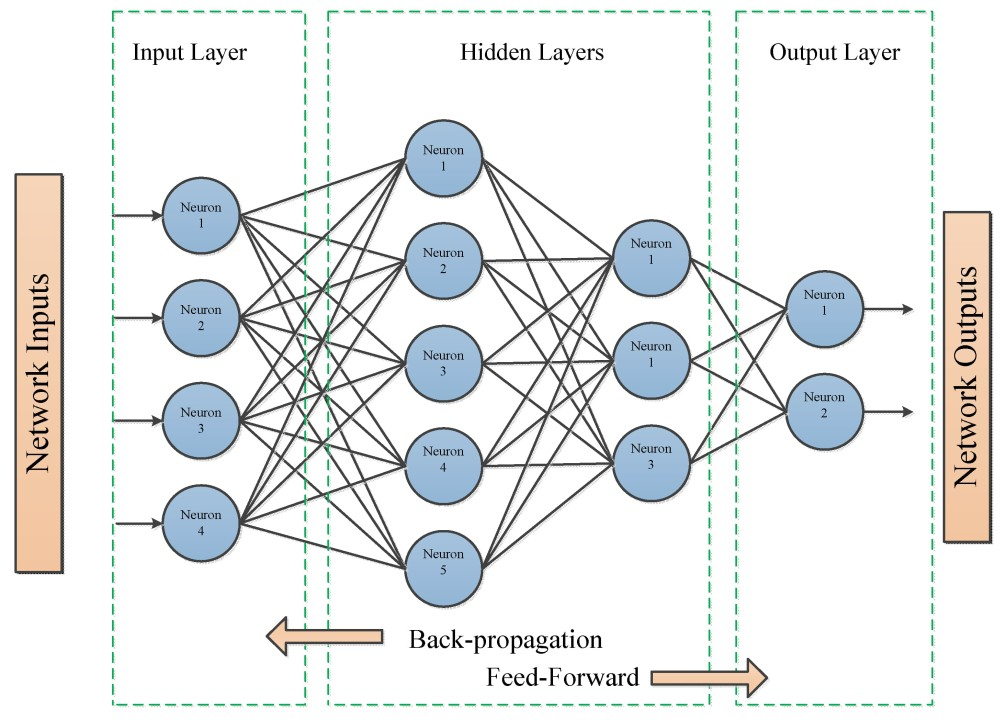
\includegraphics[width=0.7\linewidth]{resources/backpropagation.jpeg}
  \caption{Vzratno razširjanje napake. Vir:~\cite{electronics10212689}}~\label{fig:backprop}
\end{figure}

Od sedaj naprej nas bo samo zanimala evolucija uteži v procesu učenja. Na posameznih slojih bomo opazovali vektorje uteži za vsak nevron, ki jih bomo interpretirali kot točke v visoko dimenzionalnem prostoru. Za vsak sloj $i$ so to  ravno vrstice v matriki uteži $W^{(i)}$. Ker pa si visoko dimenzionalnih prostorov ne moremo predstavljati, se bomo v naslednjem razdelku ukvarjali s tem kako točke preslikati v nižje dimenzionalni prostor s čim manjšo izgubo informacij.


\chapter{Zmanjševanje dimenzionalnosti} \section{Potreba po znižanju dimenzionalnosti}
V dobi kompleksnih in visoko-dimenzionalnih podatkov je eden glavnih izzivov njihovo učinkovito razumevanje in vizualizacija. Podatkovni vektorji, kot so npr. uteži velike nevronske mreže, lahko obstajajo v prostoru z na tisoče ali celo milijone dimenzij. Za človeka (in pogosto tudi za računalniške algoritme) je tako visoke dimenzionalnosti težko neposredno obravnavati, saj si jih ne moremo predstavljati, prav tako pa se v njih pojavljajo pojavi, kot je t. i. prekletstvo dimenzionalnosti, kjer z večanjem dimenzije značilnosti podatkov postajajo razpršene in primerjave med podatki manj zanesljive. Rešitev za te težave ponujajo metode za zmanjševanje dimenzionalnosti, ki podatke preslikajo iz izvirnega visokodimenzionalnega prostora v prostor z manj razsežnostmi (npr. v dve ali tri dimenzije), pri čemer poskušajo ohraniti kar največ pomembnih informacij o podatkih. S tem postopkom lahko:
\begin{itemize}
\item lažje vizualiziramo podatke (npr. projiciramo podatke v 2D za prikaz na ravnini),
\item odstranimo šum in redundanco v podatkih ter s tem izboljšamo kakovost podatkovne predstavitve,
\item hitreje in učinkoviteje izvajamo nadaljnjo analizo ali algoritme (manj dimenzij pomeni manj računskih zahtev).
\end{itemize}
V nadaljevanju bomo predstavili tri priljubljene metode za zmanjšanje dimenzionalnosti: analizo glavnih komponent (PCA), t-SNE in UMAP. Te metode bomo uporabili tudi v naših eksperimentih kot \textit{filtrirne funkcije} v Mapper algoritmu, saj omogočajo projekcijo kompleksnih podatkov (stanj nevronske mreže med učenjem) v nižjo razsežnost, ki je primernejša za topološko analizo. \section{Analiza glavnih komponent (PCA)}
Analiza glavnih komponent (angl. \textit{Principal Component Analysis} – PCA) je klasična linearna metoda za zmanjševanje dimenzionalnosti. Osnovna ideja PCA je najti nove ortogonalne osi (smere) v podatkih, ki maksimalno pojasnijo varianco (razpršenost) podatkov. Prva glavna komponenta je smer v prostoru vhodnih podatkov, vzdolž katere imajo podatki največjo varianco. Druga glavna komponenta je smer, ki je pravokotna (ortogonalna) na prvo in pojasni čim več preostale variance, in tako naprej. Projekcijo podatkov na nekaj prvih glavnih komponent lahko nato uporabimo kot znižano-dimenzionalno predstavitev z minimalno izgubo informacij. Intuitivno si lahko postopek PCA predstavljamo tako: če imamo oblak podatkovnih točk v več-dimenzionalnem prostoru, PCA poišče smer, v katero je ta oblak najbolj razpotegnjen – to postane prva glavna komponenta. Nato poišče drugo, med seboj pravokotno smer največje razpršenosti, in tako določi drugo glavno komponento. Ko podatke projiciramo na ravnino, določeno z prvima dvema (ali prvimi nekaj) glavnima komponentama, dobimo dvodimenzionalni prikaz, ki ohranja večino raznolikosti izvirnih podatkov. PCA je uporabna za odstranjevanje redundantnih informacij in šuma v podatkih, saj pogosto le nekaj prvih komponent zajame večino variabilnosti v podatkovni množici. Metoda je tudi izračunsko razmeroma učinkovita in rezultati so deterministični (vedno enaki za iste podatke). Vendar pa je PCA omejena na linearne vzorce: če pomembne strukture v podatkih niso linearne, jih PCA ne more dobro zajeti. V takih primerih posežemo po nelinearnih metodah za zmanjšanje dimenzionalnosti, kot sta t-SNE in UMAP. \section{t-SNE (t-porazdeljeno stohastično vgrajevanje sosedov)}
t-SNE (angl. \textit{t-Distributed Stochastic Neighbor Embedding}) je nelinearna metoda za zmanjševanje dimenzionalnosti, ki je posebej priljubljena za vizualizacijo visoko-dimenzionalnih podatkov. Za razliko od PCA, ki ohranja predvsem globalno strukturo in največjo varianco, t-SNE poudari ohranjanje lokalnih razmerij med podatki. To pomeni, da t-SNE v nizki dimenziji (tipično 2D) poskuša ohraniti točke, ki so bile v originalnem prostoru med seboj blizu, še vedno tesno skupaj, medtem ko točke, ki so bile v originalu zelo daleč vsaksebi, v novi predstavitvi niso nujno na sorazmerno večji medsebojni razdalji. Algoritem t-SNE deluje tako, da najprej zgradi verjetnostno porazdelitev sosednosti med točkami v visokodimenzionalnem prostoru, nato pa skuša skonstruirati podobno porazdelitev razdalj v nizkodimenzionalnem prostoru. S postopnim optimiziranjem (gradientnim spustom) t-SNE prilagaja položaje točk v 2D/3D tako, da se porazdelitvi sosednosti v obeh prostorih čim bolje ujemata
linkedin.com
linkedin.com
. Rezultat tega procesa je nizkodimenzionalna projekcija, v kateri so si med seboj podobni podatki blizu (združeni v skupine ali gruče), kar olajša odkrivanje vzorcev in podstruktur v podatkih. t-SNE se pogosto uporablja za raziskovanje in vizualizacijo kompleksnih množic podatkov. Njegova prednost je zmožnost razkrivanja skritih skupin (grozdov) v podatkih, ki v izvirnem prostoru morda niso očitne. V našem kontekstu ga lahko uporabimo za prikaz podobnosti med različnimi stanji nevronske mreže med učenjem. Ima pa t-SNE tudi nekaj omejitev: algoritem je računsko zahteven za zelo velike množice podatkov (časovna zahtevnost hitro narašča s številom točk) in rezultati se lahko nekoliko razlikujejo ob vsaki ponovitvi (ker vključuje naključnost pri inicializaciji). Poleg tega t-SNE popači globalno strukturo podatkov – razdalje med gručami v končni projekciji ne odražajo nujno dejanskih razdalj v izvirnem prostoru. Zato iz vizualizacije t-SNE ne moremo neposredno sklepati o relativnih globalnih razdaljah med skupinami podatkov, temveč predvsem o lokalni povezanosti znotraj skupin. \section{UMAP (Uniform Manifold Approximation and Projection)}
UMAP (angl. \textit{Uniform Manifold Approximation and Projection}) je sodobna nelinearna metoda za zmanjševanje dimenzionalnosti, ki je bila razvita leta 2018
joss.theoj.org
. Po namenu je podobna t-SNE – najpogosteje se uporablja za vizualizacijo visokodimenzionalnih podatkov in iskanje vzorcev v njih. Jedro algoritma UMAP temelji na predpostavki, da podatki ležijo na večdimenzionalni mnogoterosti (manifold) nižjega reda, ki je vdelana v visokodimenzionalni prostor. UMAP skuša izslediti obliko te mnogoterosti in jo nato čim bolje “sploščiti” v manj dimenzij, pri čemer ohranja strukturo podatkov (predvsem lokalne povezave med podatki). Tehnično gledano UMAP najprej za vsako točko določi njene najbližje sosede (število sosedov je hiperparameter metode) in na podlagi razdalj do teh sosedov zgradi graf povezanosti. To določa lokalno strukturo podatkov. Nato z optimizacijskim postopkom poišče razporeditev točk v nižji dimenziji, ki kar najbolje ohranja odnose med sosednjimi točkami
linkedin.com
. Rezultat je nizkodimenzionalna predstavitev, v kateri so lokalno bližnji podatki ostali skupaj, podobno kot pri t-SNE. UMAP pa se od t-SNE razlikuje v tem, da praviloma bolje ohranja tudi globalno strukturo podatkov: gruče (skupine) podatkov v UMAP-projekciji so med seboj razporejene tako, da razdalje med njimi bolj odražajo dejanske razlike v izvirnih podatkih
linkedin.com
. Poleg tega je UMAP običajno hitrejši in bolj skalen od t-SNE, saj je zasnovan kot učinkovitejši algoritam z ozirom na velike podatkovne množice
arxiv.org
. Uporabnik lahko z izbiro hiperparametrov pri UMAP uravnava značaj projekcije. Parameter \textit{število sosedov} določa, kako “lokalno” ali “globalno” bo UMAP gledal na podatke (majhno število sosedov poudari drobne lokalne strukture, veliko število pa zajame širše vzorce). Parameter \textit{minimalna razdalja} pa vpliva na to, kako skupaj smejo biti točke v končni projekciji (višja minimalna razdalja pomeni, da bodo gruče podatkov v 2D bolj razpršene). Z izbiro teh parametrov lahko prilagodimo, ali bo vizualizacija bolj razkrila fine lokalne grozde ali pa bolj zgladila sliko v prid globalni strukturi. Ker UMAP relativno dobro ohranja različne vidike podatkovne strukture in je nezahteven za nadaljnjo uporabo, se pogosto uporablja ne le za vizualizacijo, temveč tudi kot splošna metoda za pripravo podatkov (izvleček značilk) pred nadaljnjo obdelavo v strojnem učenju. \section{Uporaba kot filtrirne funkcije v algoritmu Mapper}
Algoritem Mapper, ki ga bomo uporabili za topološko analizo učenja nevronskih mrež, zahteva izbiro ustrezne \textit{filtrirne funkcije} (angl. filter function). Ta funkcija vsakemu podatkovnemu primeru – v našem primeru trenutnemu stanju uteži nevronske mreže – priredi eno ali več številskih vrednosti. Na podlagi teh vrednosti algoritem Mapper podatke razdeli (v razponih ali intervalih) in znotraj teh podmnožic izvaja gručenje. Izbira dobre filtrirne funkcije je ključna, saj močno vpliva na končno topološko strukturo (graf) v Mapper analizi. V naših poskusih smo kot filtrirne preslikave uporabili opisane metode za zmanjševanje dimenzionalnosti. Visokodimenzionalne vektorje uteži, zajete v različnih fazah učenja nevronske mreže, smo preslikali v nižjo dimenzijo s pomočjo PCA, t-SNE in UMAP. Na primer, z metodo PCA smo vsako stanje uteži predstavili z nekaj glavnimi komponentami (pogosto že kar s prvo glavno komponento kot enodimenzionalnim filtrom). Podobno smo z metodama t-SNE in UMAP za vsako stanje uteži izračunali koordinati v dvodimenzionalnem prostoru. Ti 2D projekciji smo nato uporabili tako, da smo posamezne koordinatne osi uporabili kot ločeni filtrirni funkciji (lahko bi uporabili tudi samo eno izmed koordinat). Vsaka od teh metod ponuja nekoliko drugačen “pogled” na podatke: PCA izpostavi smer največje globalne variance v podatkih, t-SNE razkrije lokalne gruče podobnih stanj, UMAP pa skuša uravnotežiti lokalno povezanost s širšo strukturo podatkov. V naslednjih poglavjih bomo videli, kako izbira različne filtrirne funkcije vpliva na obliko in značilnosti Mapper grafov ter kaj nam ti grafi povedo o poteku učenja v nevronski mreži.

\chapter{Topološka analiza podatkov}
Topološka analiza podatkov (TDA, ang. topological data analysis) je novejša veda, ki se je začela razvijati šele v zgodnjih letih tega tisočletja. Navdih za njen razvoj izhaja iz tega, da lahko s koncepti iz topologije (vede oblik) in geometrije (vede prostora in dimenzij)  razumemo strukturo kompleksnih podatkov kot tudi nekatere podrobne in specifične informacije o njih. Ta pristop nam pomaga vizualizirati in analizirati celotno strukturo in vzorce, ki se skrivajo v podatkih, ter je manj občutljiv na majhne spremembe ali šume. TDA nam ponuja ogromno metod za analizo podatkov, ki so običajno predstavljeni v obliki oblaka oz. množice točk (ang. point cloud).

V tem poglavju bomo obravnavali nekaj osnovnih pojmov TDA, ki nam bodo kasneje v pomoč za vizualizacijo nevronske mreže s pomočjo algoritma Mapper. Defnirali bomo simplicialne komplekse in predstavili različne načine konstrukcije na podatkovnih množicah. Podali bomo Izrek o živcu, ki je glava motivacija za uporabo metod topološke analize podatkov.



\section{Glavni koraki TDA}
Kljub temu, da dandanes obstaja že veliko metod z različnimi aplikacijami, jih večina sledi naslednjim korakom:
\begin{enumerate}
    \item Vhod predstavlja končna množica točk z določeno razdaljo ali merilom podobnosti, ki je lahko osnovana na metriki okoljskega prostora (kot je evklidska v $R^d$) ali na lastni metriki, izračunani iz matrike razdalj med pari. Ta metrika je pogosto vnaprej določena ali diktirana s strani specifične uporabe. Vendar pa je izbira prave metrike ključnega pomena za odkrivanje pomembnih topoloških in geometrijskih lastnosti podatkov.
    \item Nad podatki se ustvari kontinuirana struktura, običajno preprost kompleks ali serija takih kompleksov, znana kot filtracija, ki razkriva topologijo ali geometrijo podatkov. Ti kompleksi, ki so v bistvu razširitve grafov v višje dimenzije, pomagajo prikazati strukturo podatkov na različnih ravneh. Izziv je ustvariti strukture, ki ne le natančno odražajo strukturo podatkov, ampak jih je tudi mogoče učinkovito graditi in spreminjati.
    \item Iz teh struktur se izluščijo topološke ali geometrijske podrobnosti. To lahko vključuje rekonstrukcijo osnovne oblike podatkov, na primer s triangulacijo, kar olajša dostop do njenih značilnosti, ali ustvarjanje preprostih povzetkov, ki zahtevajo specializirane metode, kot je trajna homologija, za pridobivanje nekaterih informacij. Ključna naloga tukaj je dokazati uporabnost in zanesljivost teh informacij, še posebej, kako se obnesejo v primeru napak ali šuma v podatkih.
    \item Razkrite informacije o topologiji in geometriji podatkov nudijo nove vrste značilnosti in opisov. Te lahko izboljšajo naše razumevanje podatkov, zlasti preko vizualnih metod, ali pa se integrirajo z drugimi značilnostmi podatkov za širšo analizo in aplikacije strojnega učenja. Uporaba teh informacij za ustvarjanje prilagojenih modelov analize podatkov in strojnega učenja je ključni del izkoriščanja tega, kar ponujajo orodja TDA.
\end{enumerate}

\section{Simpleks}
V nadaljevanju bomo potrebovali pojem simplicialnih kompleksov, katerih osnovni gradniki so simpleksi, ki jih bomo opisali v tem razdelku. Pri tem bomo sledili \cite{Urbančič_2020} in  Intuitivno so $n$-simpleksi geometrijski objekti z $(n + 1)$ oglišči, ki ležijo v $n$-dimenzionalnem prostoru in jih ne moremo vstaviti v nižje dimenzionalni prostor. Za gradnjo $n$-simpleksa v $n$-dimenzionalnem prostoru potrebujemo $(n + 1)$ afino neodvisnih točk.
\begin{definicija}
    Množica točk $\{x_0, \dots, x_n\}$ v vektorskem prostoru $V$ je \textbf{afino neodvisna}, če je $\{x_1 - x_0, \dots, x_n - x_0\}$ linearno neodvisna.
\end{definicija}

Matematično lahko simplekse definiramo na naslednji način.
\begin{definicija}
Naj bo \(X = \{x_0, x_1, \dots, x_n\}\) poljubna družina afino neodvisnih točk v prostoru \(\mathbb{R}^d\) za nek \(n \geq d\). Konveksno ovojnico množice \(X\),
\[
C_n(X) = C_k(x_0, x_1, \dots, x_n) = \{\sum_{i=0}^n \alpha_i x_i : \forall \alpha_i \in [0, 1], \sum_{i=0}^n \alpha_i = 1\},
\]
imenujemo \(n\)-simpleks na množici \(X\).
\end{definicija}
Točke \(X\) imenujemo oglišča \(\sigma\), simplekse ki jih razpenjajo podmnožice \(X\) pa imenujemo lica \(\sigma\).
\begin{comment}
\begin{definicija}
    Za množico \(X = \{x_0, \dots, x_k\} \subseteq \mathbb{R}^d\), \(k + 1\) afino neodvisnih točk, je \(k\)-dimenzionalni simpleks \(\sigma = [x_0, \dots, x_k]\), ki ga razpenja \(X\) konveksna ogrinjača \(X\). \\
Točke \(X\) imenujemo oglišča \(\sigma\), simplekse ki jih razpenjajo podmnožice \(X\) pa imenujemo lica \(\sigma\).
\end{definicija}
\end{comment}

Simplekse za $n = 0, 1, 2, 3$ si lahko predstavljamo vizualno.

\begin{figure}[H]
    \centering
    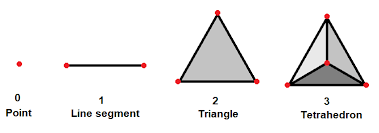
\includegraphics{slike/simplex.png}
    \caption{Simpleksi v dimenzijah 0, 1, 2 in 3. Vir: \cite{schneider_simplexes}}
    \label{fig:enter-label}
\end{figure}
\begin{comment}
    https://www.google.com/url?sa=i&url=http%3A%2F%2Fhomepages.math.uic.edu%2F~jschnei3%2FWriting%2FSimplexes&psig=AOvVaw04OUzRkF8vt7xrPuG6vtjd&ust=1714986382590000&source=images&cd=vfe&opi=89978449&ved=0CBIQjRxqFwoTCOje9KOU9oUDFQAAAAAdAAAAABAK
\end{comment}

\section{Simplicialni kompleks}
Za analizo topoloških prostorov je zelo pomembno, da jih znamo predstaviti na enostavnejši način. Za to lahko uporabljamo simplicialne komplekse, na katere lahko gledamo kot na kombinatorične opise topološkega prostora. \\
\begin{definicija}
Simplicialni kompleks \(K\) v prostoru \(R^d\) je zbirka simpleksov, tako da velja:
    \begin{enumerate}
    \item Vsako lice poljubnega simpleksa v simplicialnemu kompleksu \(K\) je tudi samo simpleks v \(K\).
    \item Naj bosta \(\sigma_1\) in \(\sigma_2\) poljubna simpleksa v \(K\). \v{C}e se sekata, potem je njun presek \(\sigma_1 \cap \sigma_2\) lice simpleksov obeh \(\sigma_1\) in \(\sigma_2\) ter je simpleks v \(K\).
\end{enumerate}
\end{definicija}

\begin{definicija}
    \textit{Geometrijski simplicialni kompleks $K$} na množici $V$ je končna množica simpleksov, ki zadoščajo naslednjima dvema pogojema:
    \begin{enumerate}
        \item Poljubno lice kateregakoli simpleksa K je simpleks v K.
        \item Presek poljubnih dveh simpleksov v K je prazna množica ali skupno lice obseh simpleksov.
    \end{enumerate}
\end{definicija}

\begin{figure}[H]
    \centering
    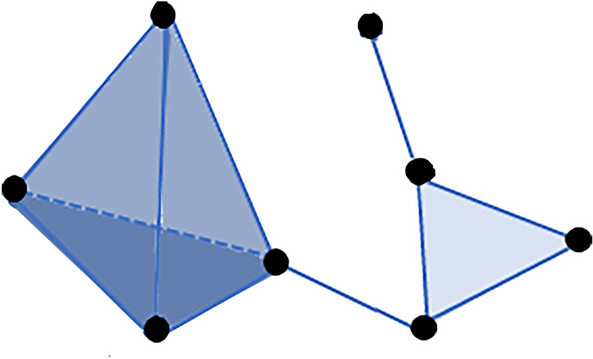
\includegraphics[width=0.8\textwidth]{slike/Simplicial-complex-eight-vertices.png}
    \caption{Simplicialni kompleks z osmimi vozlišči Vir: \cite{researchgate_simplicial_complex}}
    \label{fig:your-label}
\end{figure}
\begin{comment}
    https://www.researchgate.net/publication/358508552/figure/fig4/AS:1134810642817026@1647571349635/Simplicial-complex-An-example-of-a-simplicial-complex-composed-of-eight-vertices.png
\end{comment}

\begin{definicija}
    \textit{Abstraktni simpli\v{c}ialni kompleks} \(K\) na množici \(V\) je družina podmnožic množice \(V\), za katero velja
\[
\forall F \in K. \ G \subseteq F \implies G \in K.
\]
Množice \(F \in K\) imenujemo abstraktni simpleksi, njihovim podmnožicam \(G \subseteq F\) pa lica abstraktnega simpleksa \(F\). Dimenzijo abstraktnega simpleksa \(F\) definiramo kot \(\dim(F) = |F| - 1\). Dimenzijo abstraktnega simpli\v{c}ialnega kompleksa definiramo kot maksimalno dimenzijo njegovih simpleksov:
\[
\dim(K) = \max(\{\dim(F) \ | \ F \in K\}).
\]
\end{definicija}


\section{Gradnja simplicialnih kompleksov iz podatkov}
Simplicialne komplekse je možno zgraditi iz množice podatkov. V tem poglavju bomo opisali dva pogosto uporabljena načina. Pri tem bomo sledili \cite{10.1007/978-3-319-45378-1_1}. Privzamemo da imamo podano množico točk $X$ v metričnem prostoru $(M, d)$ in realno število $\alpha \geq 0$. Predstavili bomo dva načina, ki sta pogosto uporabljena v praksi. \cite{kun2015cech}
\begin{comment}
    https://www.jeremykun.com/2015/08/06/cech-vietoris-rips-complex/
\end{comment}

\subsection{Vietoris-Ripsov kompleks}
Prvi primer temelji na konceptu $\alpha$-soseščine. Vietoris-Ripsov kompleks $Rips_{\alpha}(\mathcal{X}) \text{ je množica simpleksov } [x_0, \ldots, x_k] \text{, tako da velja } d_{\mathcal{X}}(x_i, x_j) \leq \alpha. \text{za vse (i,j)}$. Po definiciji sledi, da je abstraktni simplicialni kompleks, v splošnem pa ne velja, da je tudi geometrični.

\subsection{Čehov kompleks}
Zelo podoben Vietoris-Ripsovem kompleksu je Čehov kompleks $C_\varepsilon$, katerega simpleksi so definirani kot množica simpleksov $[x_0, \ldots, x_k] \text{, tako da ima k + 1 zaprtih krogel} B(x_i, \alpha)$ neprazen presek.

\begin{figure}[H]
    \centering
    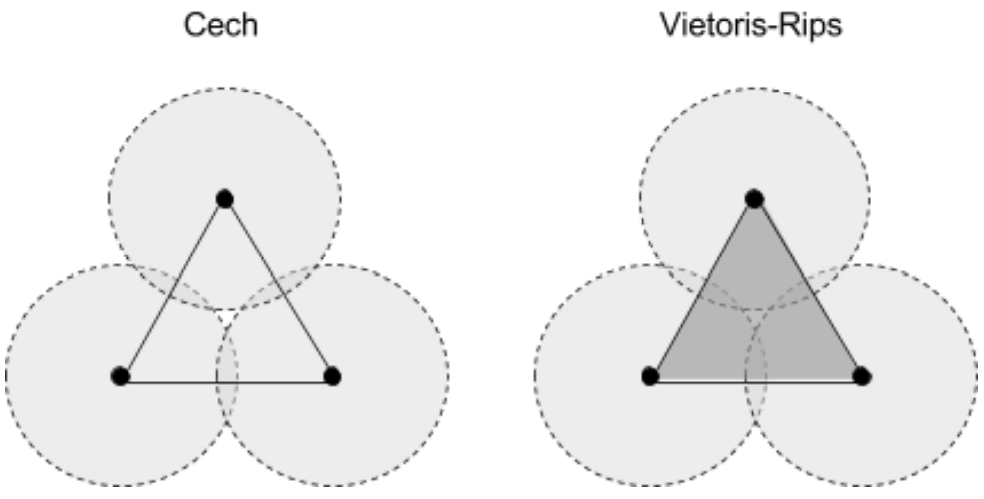
\includegraphics[width=0.7\linewidth]{slike/cech-vs-vietoris-rips-complex.png}
    \caption{Čehov in Vietoris-Ripsov kompleks. Vir: \cite{justinmath_persistent_homology}}
    \label{fig:backprop}
\end{figure}

\section{Izrek o živcu}
V tem razdelku bomo predstavili izrek o živcu, ki je osnova za Mapper algoritem, saj nam zagotavlja, da je živec, ki ga dobimo iz pokritja topološkega prostora homotopsko ekvivalenten prostoru. Izrek bomo podali brez dokaza. \cite{GuzeljBlatnik2020}

\begin{izrek}[Izrek o živcu]
Naj bo \( X \) topoološki prostor in \( \mathcal{U} = \{ U_i \}_{i \in I} \) odprto pokritje \( X \). Živec \( N(\mathcal{U}) \) pokritja \( \mathcal{U} \) je simplicialni kompleks:
\begin{itemize}
    \item Vozlišča \( N(\mathcal{U}) \) ustrezajo mnnožicam \( U_i \) v pokritju.
    \item Končna podmnožica \( \{ U_{i_0}, U_{i_1}, \ldots, U_{i_k} \} \) pokritja \( \mathcal{U} \) tvori \( k \)-simpleks v \( N(\mathcal{U}) \), če in samo če je presek \( U_{i_0} \cap U_{i_1} \cap \cdots \cap U_{i_k} \) neprazen.
\end{itemize}
Če je pokritje \( \mathcal{U} \) is \textit{dobro} (t.j., vsako končno presečišče množic v pokritju je bodisi prazno bodisi kontraktibilno), potem je topološki prostor \( X \) homotopsko ekvivalenten živcu \( N(\mathcal{U}) \). Z drugimi besedami,
\[ X \simeq N(\mathcal{U}). \]
\end{izrek}

\chapter{algoritem Mapper}
Algoritem Mapper je orodje za ekstrakcijo globalnih značilnosti iz visokodimenzionalnih podatkov, ki preoblikuje zapletene podatkovne množice v preproste simplicialne komplekse. Ti simplicialni kompleksi omogočajo kompakten globalni prikaz podatkov, neodvisno od individualnih razdalj, kotov ali točk.
Algoritem ustvarja graf, ki odraža topološko strukturo izvornega oblaka točk. Začne z izbiro zvezne funkcije, ki se imenuje filter, $f : X \rightarrow Z$, ki na primer projicira prostor $X$ na podprostor $Z$. Nato določi končno odprto pokritje $\mathcal{U} = \{U_i\}_{i \in I}$ prostora $Z$. S pomočjo algoritma za združevanje v gruče se neodvisno obdela vsaka praslika $f^{-1}(U_i)$, od koder dobimo odprto pokritje $\mathcal{V} = \{V_j\}_{j \in J}$ oblaka točk. Končni Mapperjev graf ali simplicialni kompleks je opredeljen z živcem $\mathcal{V}$, nizom podmnožic $\mathcal{K}$ iz množice $J$ z nepraznimi presečišči. Vsaka podmnožica z $n+1$ indeksi predstavlja $n$-simpleks, kjer enočlenske podmnožice tvorijo vozlišča grafa, dvodelne pa njegove robove.
\begin{comment}
https://danedmiston.github.io/home_page/assets/Mapper.pdf
\end{comment}

\cite{Langenbahn2022}
\section{Algoritem}
V nadaljevanju so opisani koraki algoritma Mapper:
\begin{algorithm}
  \caption{algoritem Mapper}\label{alg:cap}
  \begin{algorithmic}
    \State \textbf{Vhod:} Zbirka (množica) podatkov $X$ z metriko, funkcija $f: X \rightarrow \mathbb{R}$ (ali $\mathbb{R}^d$), in pokritje $\mathcal{U}$ prostora $f(X)$.
    \State \textbf{Algoritem:}
    \For{each $U \in \mathcal{U}$}
    \State Razdeli $f^{-1}(U)$  v skupine $C_{U,1}, \ldots, C_{U,k_U}$.
    \State Izračunaj živec pokritja $X$, ki ga definira $\{C_{U,1}, \ldots, C_{U,k_U}\}$ for each $U \in \mathcal{U}$.
    \EndFor
    \State \textbf{Izhod:} Simplicialni kompleks, živec (pogosto graf za dobro izbrana pokritja):
    \State \quad - Vozlišče $v_{U,i}$ za vsako skupino $C_{U,i}$.
    \State \quad - Povezava $v_{U,i}$ in $v_{U',j}$ če $C_{U,i} \cap C_{U',j} \neq \emptyset$.
  \end{algorithmic}
\end{algorithm}

\chapter{Zaključek in rezultati}

V tem poglavju si bomo pogledali metodo vizualizacije nevronske mreže in kakšne rezultate dobimo. Pri tem bomo sledili~\cite{Gabella_2021}.

Pri gradnji Mapper grafa iz nevronske mreže lahko za vsak sloj \(i\) z \(N_i\) nevroni, spremljamo evolucijo uteži nevronov, ki vstopajo vanj. Z drugimi besedami spremljamo stolpce v matriki uteži med nivojema \(i-1\) in \(i\). Nato pa za vsak korak v procesu učenja, ki ga izvedemo z metodo gradientnega spusta dobimo \(N_i\) vektorjev uteži velikosti \(N_{i-1}\), kar interpretiramo kot \(N_i\) točk v prostoru dimenzije \(N_{i-1}\). Ob koncu učenja dobimo oblak točk z \(\text{št.\ korakov} \times N_i\) točk, ki so dimenzije \(N_{i-1}\). Točke so nato s PCA projekcijo projicirane v 2-dimenzionalni prostor. Od tod potem z Mapper algoritmom zgradimo graf.

Rezultati, ki jih bomo predstavili so povzeti iz članka~\cite{Gabella_2021}. Pogledali si bomo Mapper graf nevronske mreže, ki je bila zgrajena na podatkovni zbirki MNIST.\ Gre za veliko podatkovno zbirko ročno napisanih števk (slik velikosti 28$\times$28), ki se pogosto uporablja za učenje in testiranje metod strojnega učenja.
Nevronska mreža ima dva skrita nivoja s 100 nevroni in sigmoidno aktivacijsko funkcijo. Začetne vrednosti uteži so bile nastavljene na naključne majhne vrednosti. Za filter funkcijo je bila uporabljena $L^2$ norma in DBSCAN kot algoritem gručenja.

\begin{figure}[H]
  \centering
  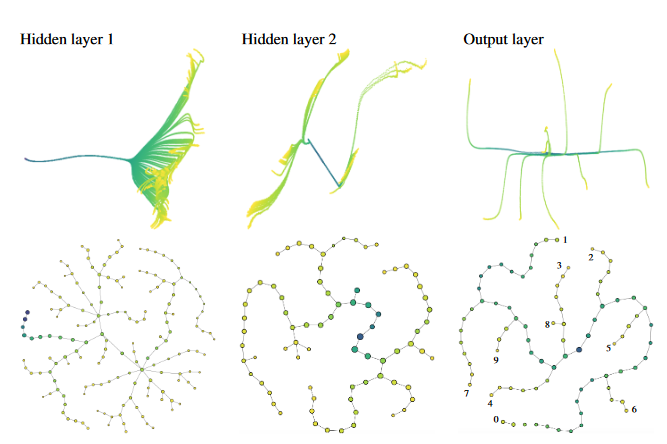
\includegraphics[width=1\linewidth]{resources/mapper-minst.png}
  \caption{Evolucija uteži učenja nevronske mreže. Vir:~\cite{Gabella_2021}}\label{fig:evolution}
\end{figure}

Z modro barvo so predstavljene uteži na začetku učenja in z rumeno na koncu. Opazimo, da se graf v zadnjem sloju razveji na 10 vej, kjer vsaka predstavlja eno izmed desetih števk. V skritem nivoju pa lahko opazimo, da se uteži nekaj časa razvijajo v enaki smeri in se šele nato razvejijo, kar bi lahko bila posledica PCA projekcije. Omenimo še, da so smeri razvejanja v različnih poskusih učenja ostale skoraj konstantne. V zadnjem sloju opazimo, da se graf že na začetku usmeri na dve nasprotni veji, ki se nato še dalje razvejita. Vidno je tudi, da so si nekatere števke zelo podobne, recimo osmica in trojka sta si zelo sorodni.


\cleardoublepage{}

%%%%%%%%%%%%%%%%%%%%%%%%%%%%%%%%%%%%%%%%
% literatura
%%%%%%%%%%%%%%%%%%%%%%%%%%%%%%%%%%%%%%%%
%\addcontentsline{toc}{chapter}{Literatura}


%\printbibliography[heading=bibintoc,type=article,title={Članki v revijah}]
%https://www.overleaf.com/project/609ce2055f917cb2f776732e
%\printbibliography[heading=bibintoc,type=inproceedings,title={Članki v zbornikih}]

%\printbibliography[heading=bibintoc,type=incollection,title={Poglavja v knjigah}]

%\printbibliography[heading=bibintoc]%,title={Celotna literatura}]

\end{document}

